\begin{minipage}{0.38\textwidth}
\begin{centering}
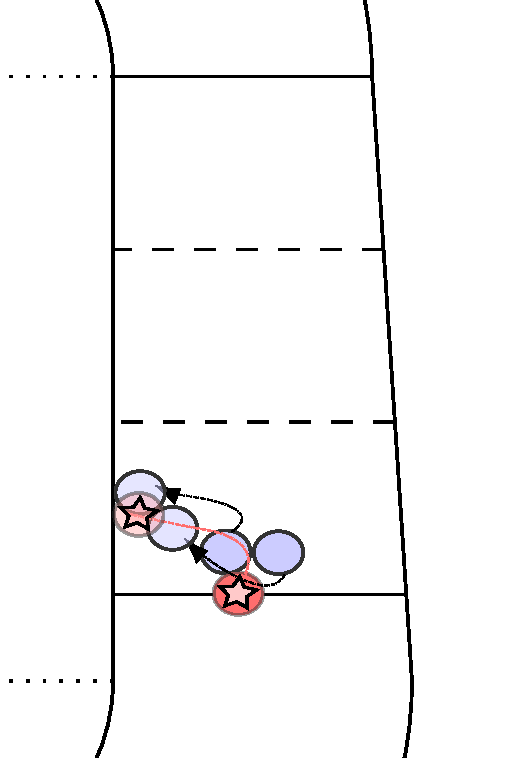
\includegraphics[scale=0.75,trim={0 1cm 0 4cm}, clip]{img/two_walls/flat_drive/chest}
{\it Blockers cede space to gain a driving position } 
\end{centering}
\end{minipage}
\hfill
\hspace{0.5cm}
\begin{minipage}{0.6\textwidth}
\subsection*{Drill: Flat Driving - Chest Drive}
\label{drill:two_wall/flat_driving}

This drill involves using a flat two wall to drive a jammer out using a chest drive. 
The main goal is for the wall to take the initiative and threaten a drive without waiting for the jammer to attempt to take a line - for this we begin by cutting off one of the jammer's lines. We distinguish between the blocker the jammer is engaged on, and the blocker that the jammer is not engaged on.
Should the jammer be pushing the seam, then one blocker can attempt to shift the jammer onto the back of the other blocker.


\end{minipage}

\begin{itemize}
\item The disengaged blocker should drop partially back while the engaged blocker should keep their back to the jammer, presenting an illegal contact zone. The engaged blocker should cede a small amount of space to improve the disengaged blocker's position while being ready to cover should the jammer attempt to take a line. The disengaged blocker's rear position cuts off their line.
\item The disengaged blocker should attempt either a hip or a low shoulder drive to rotate the jammer, then move into a chest drive. The engaged blocker should begin moving laterally. To maintain the seam, the disengaged blocker should keep their shoulder in contact with the back of the engaged jammer. During the chest-drive the engaged blocker should maintain one leg behind the jammer's position, preventing an easy escape.
\item At this point the jammer should be stood upright, ideally on toe-stops, while facing partially anti-derby and presented with either a direction or a stop block if they attempt to fight the drive, an illegal contact zone from the other blocker's back, a leg behind them preventing a disengagement without another direction, or to be pushed backwards towards a line.
\end{itemize}
